% !TeX program = xelatex
\documentclass[UTF8,11pt,a4paper,fontset=windows]{ctexart}
\usepackage[top=19mm,bottom=19mm,left=21mm,right=21mm,headheight=16pt,headsep=6mm,footskip=9mm]{geometry}
\usepackage{amsmath,amssymb,mathtools,booktabs,array,enumitem,needspace,graphicx,xcolor,fancyhdr,lastpage}
\usepackage[hidelinks]{hyperref}
\definecolor{ink}{HTML}{173F5F}
\definecolor{accent}{HTML}{227C83}
\setlength{\parindent}{0pt}
\setlength{\parskip}{4pt}
\linespread{1.12}
\setlength{\abovedisplayskip}{7pt}
\setlength{\belowdisplayskip}{7pt}
\emergencystretch=2em
\setlist{nosep,leftmargin=2em,topsep=3pt}
\newcommand{\ee}{\mathrm e}
\newcommand{\dd}{\,\mathrm d}
\newcommand{\R}{\mathbb R}
\newcommand{\ans}[1]{\boxed{#1}}
\newcommand{\q}[2]{\par\medskip\Needspace{5\baselineskip}\noindent{\large\bfseries\color{ink}第 #1 题\quad #2}\par\smallskip}
\newcommand{\tip}[1]{\par{\small\color{accent}\textbf{提示：}#1}\par}
\newcommand{\startpaper}[3]{%
\def\paperyear{#1}%
\hypersetup{pdftitle={#1学年高等数学I期中考试参考答案与详解},pdfauthor={学习资料整理}}%
\begin{center}
{\LARGE\bfseries\color{ink}高等数学 I 期中考试}\\[5pt]
{\Large #1 学年\quad 参考答案与详解}\\[6pt]
{\small 上海科技大学原卷\quad 满分 #2 分\quad #3 题\quad 整理：2026-11-10}
\end{center}
\textbf{使用说明：}题号与仓库原卷一致，题意作简要复述；解答独立编写，供学习核对，不是校方标准答案。所有角度均用弧度。
}
\pagestyle{fancy}\fancyhf{}
\fancyhead[L]{\small 高等数学 I · 历年期中详解}
\fancyhead[R]{\small\paperyear 学年}
\fancyfoot[C]{\small 第 \thepage\ 页\quad 共 \pageref{LastPage}\ 页}
\renewcommand{\headrulewidth}{0.35pt}
\raggedbottom

\begin{document}
\startpaper{2024--2025}{110}{18}
\begin{center}
\fcolorbox{accent}{white}{\parbox{.88\linewidth}{\centering
\textbf{成绩统计（用户提供，按原分数记录）}\\[3pt]
平均分：\textbf{58.32}\qquad 中位分：\textbf{57.5}}}
\end{center}
\textbf{学到洛必达法则时：}第 8 题（泰勒公式）、第 14 题（函数性态与作图）、第 17(a)（凹凸性）暂时跳过。第 17(b) 给出仅用罗尔定理的解法；第 18 题为综合选做。详见仓库复习目录。

\textbf{选择、填空速查}
\begin{center}
\begin{tabular}{c*{5}{c}}
\toprule 题号 & 1 & 2 & 3 & 4 & 5\\\midrule
答案 & C & C & C & C & A\\\bottomrule
\end{tabular}
\end{center}
\begin{tabular}{@{}cl@{}}
6 & $f^{-1}(u)=\begin{cases}\arccos(-u),&-1\le u<0,\\-\sqrt u,&u>0;\end{cases}$\quad 定义域 $[-1,0)\cup(0,+\infty)$。\\[7pt]
7 & $1/2$。\\[4pt]
8 & $\sin^2x=x^2-\frac13\cos(2\xi)x^4$，$\xi$ 介于 $0$ 与 $x$ 之间。\\[4pt]
9 & $3$ 个。\\[4pt]
10 & $2024!\,3^{2024}\frac{\sqrt3}2$。\\
\end{tabular}

\q{1}{实根个数：C（$3$ 个）}
设 $F(x)=2^x-x^2-1$。有 $F(0)=F(1)=0$，又 $F(4)=-1<0$、$F(5)=6>0$，故 $(4,5)$ 中至少还有一个零点，已有三个不同实根。

另一方面 $F'''(x)=(\ln2)^3 2^x>0$。若有四个不同实根，连续三次应用罗尔定理，必有某点 $F'''(x)=0$，矛盾。所以恰有三个实根。
\tip{本题可以用罗尔定理完成，无须函数极值或凹凸性知识。}

\q{2}{分段函数的二阶可导性：C}
原函数为 $f(x)=\frac x2\sin\frac x2$（$x\le0$），$f(x)=x\sin x$（$x>0$）。由差商可得 $f'(0)=0$，且
\[
f'(x)=\begin{cases}\frac12\sin\frac x2+\frac x4\cos\frac x2,&x<0,\\0,&x=0,\\\sin x+x\cos x,&x>0.\end{cases}
\]
$f'(x)\to0=f'(0)$，故一阶导函数连续；但
\[
\lim_{h\to0^-}\frac{f'(h)-f'(0)}h=\frac12,\qquad
\lim_{h\to0^+}\frac{f'(h)-f'(0)}h=2,
\]
所以 $f''(0)$ 不存在。选 C。

\newpage
\q{3}{数列的最大值、最小值：C}
令 $r_n=(1+3^n)^{1/n}$，则 $3<r_n\le4$，且 $r_n\to3$；$x_n=r_n-(-1)^n/n$。
对奇数 $n$，$x_n=r_n+1/n\le5$；对偶数 $n$，$x_n=r_n-1/n<4$。由 $x_1=5$，最大值为 $5$。

偶数 $n\ge4$ 时，$x_n>3-1/n\ge11/4$；奇数 $n$ 时，$x_n>3$。而
$x_2=\sqrt{10}-1/2<11/4$，因此最小值为 $\sqrt{10}-1/2$。两者均存在，选 C。

\q{4}{极限函数的不可导点：C}
若 $|x|\le1$，由 $1\le(1+|x|^{3n})^{1/n}\le2^{1/n}$ 得极限为 $1$。
若 $|x|>1$，提出 $|x|^{3n}$ 得极限为 $|x|^3$。所以
\[
f(x)=\begin{cases}1,&|x|\le1,\\|x|^3,&|x|>1.\end{cases}
\]
在 $x=-1$ 处左右导数为 $-3,0$，在 $x=1$ 处为 $0,3$；其余点可导。因此恰有两个不可导点。

\q{5}{原函数与反函数：A}
\textbf{A 正确：}在 $0$ 处可导必连续。

\textbf{C 不一定：}从恒等函数出发，只交换 $1,2$ 两点的函数值。所得函数仍是 $\R$ 到 $\R$ 的双射，且在 $0$ 处可导，但不严格单调。

\textbf{D 不一定：}取 $f(x)=x^3$，其导函数连续，而反函数 $\sqrt[3]x$ 在 $0$ 处不可导。原函数导数还需要非零等条件，才能保证反函数可导。

\textbf{B 也不一定（补充构造，可略读）：}“只在 $0$ 可导”没有提供邻域内的连续性，不能直接套用连续单调函数的反函数定理。下面给出一个完整反例。
对 $n\ge2,k\ge0$，令
\[
t_{n,k}=2^{-n}+2^{-2n-k},\qquad s_{n,k}=2^n(2k+1).
\]
各 $t$ 点互异、各 $s$ 点互异，且两类点不相交。定义
\[
f(t_{n,k})=t_{n,k+1},\quad f(s_{n,0})=t_{n,0},\quad
f(s_{n,k+1})=s_{n,k},
\]
其余实数取 $f(x)=x$。在每条链上，每点恰有一个像和一个原像，因此是双射，且 $f(0)=0$。
趋近 $0$ 的修改点只能来自 $t$ 类；在这些点
\[
\left|\frac{f(t_{n,k})}{t_{n,k}}-1\right|\le2^{-n-1}\longrightarrow0,
\]
故 $f'(0)=1$。但 $t_{n,0}\to0$，而 $f^{-1}(t_{n,0})=2^n\to+\infty$，反函数在 $0$ 处不连续。

\newpage
\q{6}{反函数及其定义域}
$x<0$ 时 $u=x^2>0$，反解应取 $x=-\sqrt u$。
$0\le x<\pi/2$ 时 $u=-\cos x\in[-1,0)$，反解为 $x=\arccos(-u)$。
两段值域不重叠，所以
\[
\ans{f^{-1}(u)=\begin{cases}\arccos(-u),&-1\le u<0,\\-\sqrt u,&u>0,\end{cases}
\quad D_{f^{-1}}=[-1,0)\cup(0,+\infty).}
\]
\tip{$0$ 不在原函数值域内，因此反函数在 $u=0$ 没有定义。}

\q{7}{由已知极限求另一极限：$1/2$}
记 $A(x)=(\cos x-1+f(x))/x^3\to1$，则
\[
\frac{f(x)}{\sin^2x}
=A(x)\frac{x^3}{\sin^2x}+\frac{1-\cos x}{\sin^2x}
\longrightarrow 1\cdot0+\frac12=\ans{\frac12}.
\]
这里 $x^3/\sin^2x=x(x/\sin x)^2\to0$，而 $(1-\cos x)/\sin^2x=1/(1+\cos x)\to1/2$。无需展开。

\q{8}{三阶麦克劳林公式（本次范围外）}
对 $f(x)=\sin^2x=(1-\cos2x)/2$，有
\[
f(0)=f'(0)=f'''(0)=0,\quad f''(0)=2,\quad f^{(4)}(x)=-8\cos2x.
\]
故带拉格朗日余项的三阶公式为
\[
\ans{\sin^2x=x^2-\frac13\cos(2\xi)x^4,\quad\xi\text{ 介于 }0\text{ 与 }x\text{ 之间}.}
\]
三阶多项式的三次项系数可以为零；“三阶公式”的余项使用四阶导数。

\q{9}{第二类间断点：$3$ 个}
原函数为 $f(x)=\frac{\ln|x+1|}{(1+\ee^{1/(x-2)})(x-3)}\sin\frac1{x-1}$，只需检查 $-1,1,2,3$。
\begin{itemize}
\item $x=-1$：对数趋于 $-\infty$，其余乘因子趋于非零常数，是第二类间断点。
\item $x=1$：正弦因子振荡，前面的系数趋于非零常数，是第二类间断点。
\item $x=2$：左极限为 $-\ln3\sin1$，右极限为 $0$。两者有限但不同，是第一类跳跃间断点。
\item $x=3$：$x-3$ 以外的因子趋于非零常数，出现无穷间断，是第二类间断点。
\end{itemize}
因此第二类间断点共 $\ans{3}$ 个，不能把 $x=2$ 也算进去。

\q{10}{高阶导数：$2024!\,3^{2024}\sqrt3/2$}
因 $y=(x-1)^{2024}(x+2)^{2024}\sin(\pi x/3)$，在 $x=1$ 求 $2024$ 阶导数时，乘积公式中只有对 $(x-1)^{2024}$ 求满 $2024$ 次导数的一项非零。因此
\[
\ans{y^{(2024)}(1)=2024!\,3^{2024}\sin\frac\pi3=2024!\,3^{2024}\frac{\sqrt3}2.}
\]
本题使用高阶乘积求导，不需要泰勒公式。

\newpage
\q{11}{三角函数极限：$1/6$}
使用和差化积，避免泰勒展开：
\[
\cos(\sin x)-\cos x
=2\sin\frac{x+\sin x}2\sin\frac{x-\sin x}2.
\]
由洛必达法则，
\[
\lim_{x\to0}\frac{x-\sin x}{x^3}
=\lim_{x\to0}\frac{1-\cos x}{3x^2}=\frac16.
\]
因 $(x+\sin x)/x\to2$，用 $\sin u/u\to1$ 得
\begin{align*}
\frac{\cos(\sin x)-\cos x}{\sin^4x}
={}&\frac12\frac{\sin\frac{x+\sin x}2}{\frac{x+\sin x}2}
\frac{\sin\frac{x-\sin x}2}{\frac{x-\sin x}2}
\frac{x+\sin x}{x}\frac{x-\sin x}{x^3}
\left(\frac{x}{\sin x}\right)^4\\
&\longrightarrow\frac12\cdot1\cdot1\cdot2\cdot\frac16\cdot1=\ans{\frac16}.
\end{align*}

\q{12}{隐函数的二阶导数：$-\ee^{-1}$}
方程为 $\ee^{x+y}-\cos(xy)=\ee-1$。取 $x=0$ 得 $\ee^{y(0)}=\ee$，故 $y(0)=1$。
求一次导数：
\[
\ee^{x+y}(1+y')+\sin(xy)(y+xy')=0.
\]
在 $(0,1)$ 处得到 $y'(0)=-1$。再次求导：
\begin{align*}
&\ee^{x+y}\bigl((1+y')^2+y''\bigr)
+\cos(xy)(y+xy')^2\\
&\hspace{35mm}+\sin(xy)(2y'+xy'')=0.
\end{align*}
代入 $x=0,y=1,y'=-1$ 得 $\ee\,y''(0)+1=0$，故 $\ans{y''(0)=-1/\ee}$。

\q{13}{参数曲线的二阶导数：$\sqrt2$}
由 $y(t)=\ln(t+\sqrt{1+t^2})$ 得 $y_t=1/\sqrt{1+t^2}$。因此
\[
\frac{\dd y}{\dd x}=\frac{y_t}{x_t}=\sqrt{1+t^2}
\quad\Longrightarrow\quad x_t=\frac1{1+t^2}.
\]
由于 $\arctan t$ 的导数也是 $1/(1+t^2)$，由中值定理，$x(t)-\arctan t$ 为常数。
利用 $x(0)=0$ 得 $x(t)=\arctan t$。所以 $x=\pi/4$ 对应 $t=1$，而
\[
\frac{\dd^2y}{\dd x^2}
=\frac{\frac{\dd}{\dd t}\sqrt{1+t^2}}{x_t}
=\frac{t/\sqrt{1+t^2}}{1/(1+t^2)}=t\sqrt{1+t^2}.
\]
故 $\ans{\left.\frac{\dd^2y}{\dd x^2}\right|_{x=\pi/4}=\sqrt2}$。
\tip{找 $x(t)$ 也无需积分：比较导数，再用“导数恒为零则函数为常数”。}

\newpage
\q{14}{函数性态与作图（本次范围外）}
设 $f(x)=(x+2)\ee^{1/x}$。

\textbf{定义域、间断与零点。}定义域为 $\R\setminus\{0\}$，且
\[
\lim_{x\to0^-}f(x)=0,\qquad\lim_{x\to0^+}f(x)=+\infty.
\]
故 $x=0$ 是间断点。指数因子始终为正，唯一零点为 $x=-2$。

\textbf{单调性与极值。}原卷给出
\[
f'(x)=\frac{(x+1)(x-2)}{x^2}\ee^{1/x}.
\]
分母和指数因子均为正，故只需检查 $(x+1)(x-2)$ 的符号：
\begin{center}
\begin{tabular}{c*{4}{c}}
\toprule 区间 & $(-\infty,-1)$ & $(-1,0)$ & $(0,2)$ & $(2,+\infty)$\\\midrule
$f'$ & $+$ & $-$ & $-$ & $+$\\
$f$ & 递增 & 递减 & 递减 & 递增\\\bottomrule
\end{tabular}
\end{center}
因此极大值点为 $(-1,\ee^{-1})$，极小值点为 $(2,4\sqrt\ee)$。

\textbf{值域。}负半轴上，函数由 $-\infty$ 上升到 $\ee^{-1}$ 再趋向 $0$；正半轴上，两端均趋向 $+\infty$，在 $x=2$ 取得最小值。因此
\[
\ans{\text{值域}=(-\infty,\ee^{-1}]\cup[4\sqrt\ee,+\infty).}
\]

\textbf{凹凸性与拐点。}为避免术语差异，这里明确以 $f''>0$ 为下凸（开口向上）、$f''<0$ 为上凸（开口向下）。由
\[
f''(x)=\frac{5x+2}{x^4}\ee^{1/x}
\]
可得：上凸区间为 $(-\infty,-2/5)$，下凸区间为 $(-2/5,0)$ 与 $(0,+\infty)$。
在 $x=-2/5$ 处二阶导数变号，拐点为
\[
\ans{\left(-\frac25,\frac85\ee^{-5/2}\right)}.
\]
$x=0$ 不属于定义域，因此不是拐点。

\textbf{渐近线。}因右极限为 $+\infty$，竖直渐近线为 $x=0$。又
\[
\lim_{x\to\pm\infty}\frac{f(x)}x=1,\qquad
\lim_{x\to\pm\infty}(f(x)-x)
=\lim_{x\to\pm\infty}\left[x(\ee^{1/x}-1)+2\ee^{1/x}\right]=3,
\]
所以两端共用斜渐近线 $\ans{y=x+3}$，没有水平渐近线。
\tip{极大、极小是局部概念；本函数在整个定义域上既无最大值，也无最小值。图见下一页。}

\newpage
\q{14（续）}{函数草图}
\begin{center}
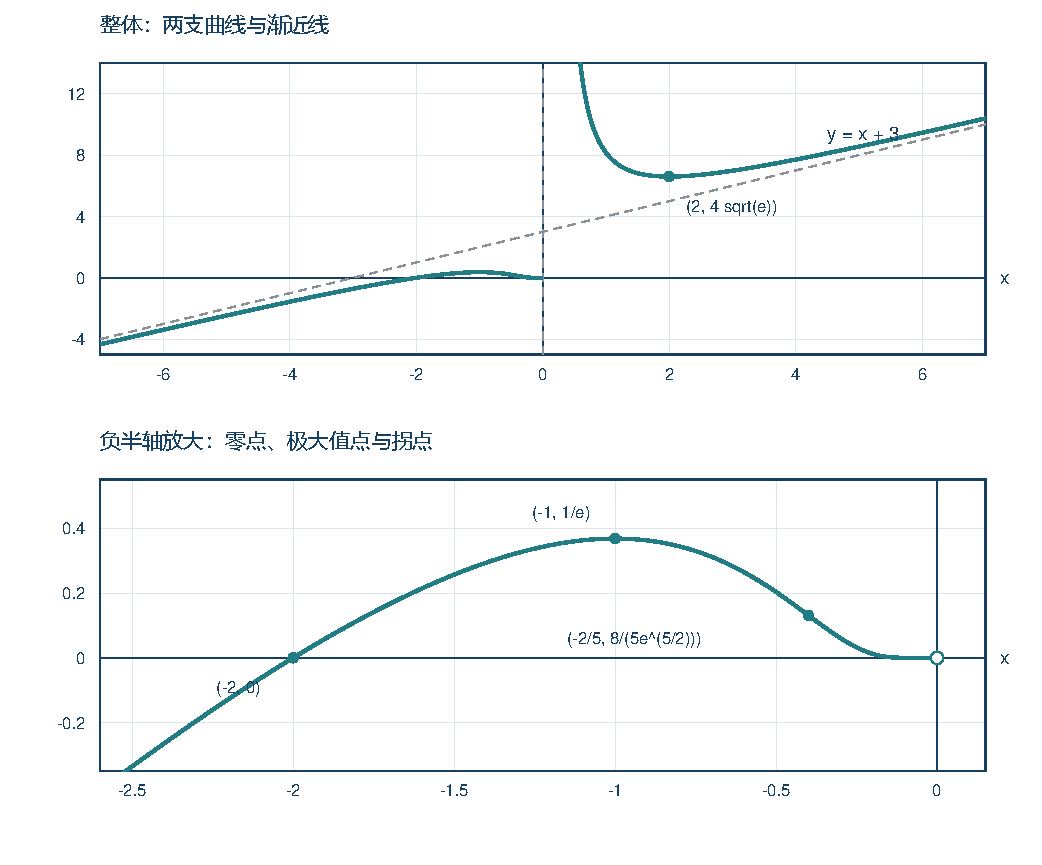
\includegraphics[width=\linewidth]{function-24-q14.pdf}
\end{center}
上图是整体示意，下图放大负半轴分支；虚线为渐近线，空心圆表示 $(0,0)$ 不属于曲线。正半轴靠近 $0$ 时曲线向上无界，超出显示窗口。

\q{15}{用定义证明函数趋于正无穷}
要证 $\lim_{x\to1}1/(x-1)^2=+\infty$。对于任意 $M>0$，取
\[
\delta=\frac1{\sqrt M}>0.
\]
只要 $0<|x-1|<\delta$，就有
\[
\frac1{(x-1)^2}>\frac1{\delta^2}=M.
\]
这正是函数趋于 $+\infty$ 的定义，故得证。
\tip{原题称“$\varepsilon$--$\delta$ 语言”；对于无穷极限，严格写法是 $M$--$\delta$：任给高度阈值 $M>0$，找到对应邻域。}

\newpage
\q{16}{斐波那契比值数列}
已知 $a_1=a_2=1$、$a_{n+2}=a_n+a_{n+1}$，令 $b_n=a_n/a_{n+1}$。所有 $a_n>0$，所以
\[
b_{n+1}=\frac1{1+b_n},\qquad
b_{n+2}=\frac{1+b_n}{2+b_n}=:T(b_n).
\]
记 $\alpha=(\sqrt5-1)/2$，它满足 $\alpha^2+\alpha=1$、$T(\alpha)=\alpha$。
而
\[
T'(t)=\frac1{(2+t)^2}>0\quad(t>0),\qquad
T(t)-t=\frac{1-t-t^2}{2+t}.
\]

\textbf{(a) 奇偶子列单调性。}
初值 $b_1=1>\alpha$、$b_2=1/2<\alpha$。
若 $0<t<\alpha$，则 $1-t-t^2>0$，故 $T(t)>t$；再由 $T$ 严格增加，得 $T(t)<T(\alpha)=\alpha$。
若 $t>\alpha$，同理有 $\alpha<T(t)<t$。
逐次应用在奇、偶子列上即得
\[
\frac12=b_2<b_4<b_6<\cdots<\alpha
<\cdots<b_5<b_3<b_1=1.
\]
所以偶数子列严格上升，奇数子列严格下降。

\textbf{(b) 收敛及其极限。}两条子列分别单调有界，故均存在有限正极限，设为 $\ell_e,\ell_o$。
对两步递推式 $b_{n+2}=T(b_n)$，在奇、偶下标上分别取极限，得
\[
\ell_e=T(\ell_e),\qquad \ell_o=T(\ell_o).
\]
正数 $\ell$ 若满足 $\ell=(1+\ell)/(2+\ell)$，则 $\ell^2+\ell-1=0$，唯一正根为 $\alpha$。
所以 $\ell_e=\ell_o=\alpha$，由奇偶子列同极限，得到
\[
\ans{\lim_{n\to\infty}b_n=\frac{\sqrt5-1}2}.
\]
\tip{不能只证明两条子列各自收敛就直接宣布原数列收敛；还必须说明它们的极限相同。}

\newpage
\q{17}{线性插值的误差界}
设 $|f''(x)|\le1$（$0<x<1$），且
\[
g(x)=f(x)-f(0)(1-x)-f(1)x.
\]
有 $g(0)=g(1)=0$、$g''(x)=f''(x)$。结论的取值范围为 $x\in[0,1]$。

\textbf{(a) 下凸性（本次范围外，可跳过）。}令
\[
h(x)=g(x)-\frac{x(1-x)}2.
\]
则 $h''(x)=f''(x)+1\ge0$，因此 $h$ 下凸，且 $h(0)=h(1)=0$。

\textbf{(b) 标准解法。}下凸函数的图像在端点连线下方，因此 $h(x)\le0$，得到
$g(x)\le x(1-x)/2$。另一方面，令 $k(x)=g(x)+x(1-x)/2$，有
$k''(x)=f''(x)-1\le0$；其图像在端点连线上方，因此 $k(x)\ge0$，即 $g(x)\ge-x(1-x)/2$。综上
\[
|g(x)|\le\frac{x(1-x)}2\le\frac18.
\]

\textbf{(b) 只用罗尔定理的解法（当前范围可做）。}
固定任意 $u\in(0,1)$，令
\[
C=\frac{g(u)}{u(u-1)},\qquad H(t)=g(t)-Ct(t-1).
\]
则 $H(0)=H(u)=H(1)=0$。分别在 $[0,u]$、$[u,1]$ 上用罗尔定理，存在
$\eta_1\in(0,u)$、$\eta_2\in(u,1)$ 使 $H'(\eta_1)=H'(\eta_2)=0$。
再对 $H'$ 在 $[\eta_1,\eta_2]$ 上应用罗尔定理，存在 $\xi\in(\eta_1,\eta_2)$ 使
\[
0=H''(\xi)=f''(\xi)-2C.
\]
故 $C=f''(\xi)/2$，于是
\[
|g(u)|=\frac{|f''(\xi)|}2\,u(1-u)
\le\frac{u(1-u)}2\le\ans{\frac18}.
\]
端点 $u=0,1$ 时 $g(u)=0$，也满足结论。由于 $f$ 二阶可导，$H'$ 在上述内部闭区间连续、开区间可导，第二次应用罗尔定理的条件成立。

\textbf{界的精确性。}例如 $f(x)=x^2/2$ 时，$g(x)=-x(1-x)/2$，在 $x=1/2$ 取到 $|g(x)|=1/8$。所以常数 $1/8$ 不能进一步缩小。

\newpage
\q{18}{贝塞尔曲线（综合选做）}
以下把 $P_i=(x_i,y_i)$ 看成平面向量。题目已给出递推定义，因此无需事先学习贝塞尔曲线；需要向量代数、求导与数学归纳法。

\textbf{(1) 一次曲线。}由定义
\[
\ans{B_{P_0P_1}(t)=(1-t)P_0+tP_1,\quad0\le t\le1.}
\]
即 $x(t)=(1-t)x_0+tx_1$，$y(t)=(1-t)y_0+ty_1$。它是从 $P_0$ 到 $P_1$ 的\textbf{闭线段}，随参数增加匀速走过，包含两端点。

\textbf{(2) 二次曲线的二阶导数。}再用一次递推，得
\[
B(t)=(1-t)^2P_0+2t(1-t)P_1+t^2P_2.
\]
因此
\[
\ans{B''(t)=2(P_0-2P_1+P_2)
=\bigl(2(x_0-2x_1+x_2),\,2(y_0-2y_1+y_2)\bigr).}
\]

\textbf{(3) 非共线时是一段抛物线。}记 $v=2(P_1-P_0)$、$a=P_0-2P_1+P_2$，则
$B(t)=P_0+vt+at^2$。
非共线意味着 $v,a$ 线性无关，尤其 $a\ne0$。作平移、旋转，令纵轴沿 $a$ 的方向；新坐标中
\[
X=v_Xt,\qquad Y=v_Yt+|a|t^2,\qquad v_X\ne0.
\]
消去 $t=X/v_X$：
\[
Y=\frac{v_Y}{v_X}X+\frac{|a|}{v_X^2}X^2.
\]
二次项系数非零，故轨迹是非退化抛物线；$0\le t\le1$ 取其中一段。这也对应恒定加速度运动，非共线条件排除了直线轨迹。

\textbf{(4) 显式公式的归纳证明。}当 $n=0$ 时公式就是 $B_{P_0}=P_0$。假设 $n-1$ 次公式成立，代入递推：
\begin{align*}
B_{P_0\cdots P_n}(t)
={}&\sum_{i=0}^{n-1}\binom{n-1}{i}(1-t)^{n-i}t^iP_i\\
&+\sum_{i=1}^{n}\binom{n-1}{i-1}(1-t)^{n-i}t^iP_i.
\end{align*}
中间项由帕斯卡恒等式 $\binom{n-1}{i}+\binom{n-1}{i-1}=\binom ni$ 合并；首末两项也分别有系数 $1$，于是
\[
\ans{B_{P_0\cdots P_n}(t)=\sum_{i=0}^n\binom ni(1-t)^{n-i}t^iP_i.}
\]
由数学归纳法，结论对所有非负整数 $n$ 成立，端点值按多项式的连续取值理解。
\end{document}
